\chapter{Recerca prèvia}
\label{c:recerca prèvia}
\section{La Història de la IA: Des dels orígens fins avui}
\begin{enumerate}
     \item \textbf{El Naixement d'una Idea Revolucionària (1956)}

             Alan Turing, el geni matemàtic que va desxifrar Enigma, una màquina emprada pels nazis per codificar els seus missatges durant la Segona Guerra Mundial (1939-1945), va fer una pregunta provocadora a la comunitat científica: "Podran les màquines pensar alguna vegada?". Aquesta qüestió va obrir les portes a un nou camp d’estudi. En 1956 John McCarthy, Marvin Minsky i d'altres especialistes van nominar oficialment el terme ``intel·ligència artificial'' durant la conferència de Dartmouth, marcant l'inici d'una nova era tecnològica.

      \item \textbf{El Joc que ho va canviar tot: The Imitation Game/El test de Turing}

            L'origen de la IA es basa en un experiment molt senzill, però profund: El joc d'imitació (The imitation game), proposat per Alan Turing. Per respondre a la pregunta "Podran les màquines pensar alguna vegada?", Turing va dissenyar un joc que funcionava com a test per les màquines anomenat ``The Imitation Game''. Aquest test consistia a fer que un avaluador havia d'intercanviar textos escrits amb una persona i una màquina durant 5 minuts, aquest avaluador no sabia qui era qui i havia d'esbrinar qui era l'humà. Si la màquina aconseguia enganyar a l'avaluador passava el test i es considerava que la màquina havia aconseguit un nivell de comportament lingüístic equivalent al d'un humà, per tant, podríem considerar que les màquines poden pensar. Aquest joc ha estat evolucionant gràcies als avenços de la ciència i de la tècnica, i encara avui dia és conegut com el test de Turing.

     \item Les grans fites de la IA
        \subsubsection{1997: La màquina que va vèncer un campió}
            La supercomputadora Deep Blue desenvolupada per IBM va derrotar el campió mundial d’escacs, Garri Kaspàrov, demostrant que la IA podia superar els humans en jocs d’estratègia complexos.
        \subsubsection{2022: L'explosió de la IA}
         Milions d’usuaris van descobrir models com ChatGPT que podien escriure, traduir i programar amb un llenguatge gairebé humà, obrint nous horitzons en la interacció home-màquina.
        \subsubsection{2025: La IA en tots els àmbits}
        2025: La IA en Tots els Àmbits
        Avui, la IA està present en dibuix, contingut audiovisual, cotxes autònoms, medicina i molt més, amb models cada vegada més especialitzats i avançats.

\end{enumerate}

(Fonts:~\cite{McCarthy_Minsky_Rochester_Shannon_2006},~\cite{deepblue},
~\cite{chatGPT2022} i~\cite{10.1093/mind/LIX.236.433})


\section{Que és la IA?}
% Hem estat parlant molt durant aquest treball sobre la IA, i ara que em après quina és la seva història, hem de saber que és. \\
% Doncs bé, p
Podem definir la IA com sistemes de software i de hardware dissenyats per humans que actuen en la dimensió física o digital, és a dir, raonar sobre el coneixement, processant la informació derivada de dades i prendre les millors decisions per assolir l'objectiu donat. O dit d'un altra manera, és un camp de la informàtica que consisteix en un conjunt de capacitats intel·lectuats i cognitives expressades per un sistema informàtic creat pels humans, que té com a propòsit imitar la intel·ligència humana. \\

Un exemple d'IA i que tot el món coneix i utilitza és el ChatGPT, un xatbot impulsat per un model d'intel·ligència artificial generativa de l'empresa OpenAI. Fa servir tècniques de processament de llenguatge natural per comprendre preguntes fetes per l'usuari i generar respostes coherents en converses, simulant una interacció similar a la d'un humà. També pot generar o editar imatges, processar àudios, llegir arxius i molt més.

\section{Com funciona la IA?}
Una vegada que ja sabem que és una IA, ens toca entendre com funciona.
Les intel·ligències artificials utilitzen algoritmes i models matemàtics per processar grans quantitats de dades
i prendre accions basades en patrons i regles establertes a través de l'aprenentatge automàtic o l'aprenentatge profund.
Per tant, per funcionar necessitarà:

\begin{enumerate}
    \item \textbf{Dades}\\
    Les dades són fonamentals per la IA, ja que és la base de l'aprenentatge del model, per poder raonar, prendre decisions, i millorar la precisió. Aquí esdevenen uns exemples que pot haver-hi:
         \begin{itemize}
            \item \textbf{Base d'aprenentage}\\
            Els algoritmes de la IA necessiten a base de dades i una gran diversitat de dades per poder identificar patrons i construir prediccions.

           \item \textbf{Qualitat vs Quantitat}\\
            Una gran quantitat de dades ajudaran la IA a obtenir major precisió, però la qualitat és encara més important per la complexitat de dades que aporta, això evitarà que la IA cometes errors per informació incompleta.\textbf{ Per exemple:} En l'àmbit mèdic si vols que la IA faci una predicció i tan sols li dones una quantitat important de persones sanes i no d'altres exemplars, la IA simplement descartarà d'altres possibilitats que podrien haver-hi i només agafar la sana.

            \item \textbf{Exemples Reals}\\
            Els sistemes dels cotxes o assistents virtuals necessiten dades en temps reals per adaptar-se de l'entorn, també plataformes com Netflix o Spotify necessiten dades personalitzades per poder generar recomanacions amb precisió.
          \end{itemize}

    \item \textbf{Algorismes}\\
  Totes les aplicacions de la IA tenen el propòsit de capacitar la màquina perquè puguin operar com un humà. Tot això està basat en combinacions de diferents tipus d’algorismes. A continuació, explicarem els diferents tipus d’algorismes d’aprenentatge.
        \begin{itemize}
           \item \textbf{L'aprenentage automàtic(Machine learning)}\label{Aprenentatge_automàtic}
            És una branca crucial de la intel·ligència artificial, consisteix a cobrar vida a la màquina, donar-li el poder d'aprendre com els humans, executar tasques de manera autònoma i finalment, les infinites possibilitats d'evolucionar a través de l'experiència i molt més. Segons la UC Berkeley~\cite{Berkeley} el procés de l'aprenentatge automàtic és

            {\color{gray}
            \item \textbf{Mecanisme de predicció}
            \subitem\hspace*{-1\leftmargin} Un conjunt de regles o operacions matemàtics que analitza   les dades d'entrada i intenta identificar els patrons que busca el model.
            \item \textbf{Algoritme d'optimització}
            \subitem\hspace*{-1\leftmargin} El procés que ajusta automàticament el model per minimitzar l'error, modificant els paràmetres interns per millorar les prediccions futures.}
        \end{itemize}

             Segons Nvidia~\cite{Nvidia}, hi ha molts tipus d'aprenentatge automàtics:
            \begin{enumerate}
                \item \textbf{Aprenentatge supervisat}
                 L'aprenentatge supervisat és un tipus d'aprenentatge automàtic que treballa amb dades etiquetades, és a dir, dades que ja inclouen la solució o resultat desitjat. En aquest mètode, la intel·ligència artificial aprèn a associar les dades d'entrada amb les seves etiquetes corresponents, mitjançant l'anàlisi d'exemples prèviament resolts. Això li permet desenvolupar la capacitat de resoldre problemes nous aplicant la lògica i els patrons identificats a partir de dades reals.
                 \begin{comment}
                \textbf{Avantatges i desavanantatge:}
                 Aquest mètode destaca per la seva alta precisió en problemes ben definits, ja que al treballar   amb dades prèviament etiquetades pot assolir bons resultats en tasques de classificació i regressió. Una altra avantatge important és la facilitat per avaluar el rendiment dels models. A més, es tracta d'una àmplia àrea d'estudi amb una gran varietat d'algoritmes ben desenvolupats i optimitzats, com ara els arbres de decisió, els random forests, les màquines de vectors de suport (SVM) o les xarxes neuronals. Finalment, un cop entrenat adequadament, el model pot generalitzar el seu aprenentatge i fer prediccions útils sobre dades noves.\\

                 No obstant això, aquest enfocament també presenta alguns inconvenients significatius. El principal desavantatge és la seva forta dependència de conjunts de dades etiquetades, que sovint són costosos d'obtenir i preparar com las de medicines. Un altre problema freqüent és el sobreajustament (overfitting), que ocorre quan el model memoritza les dades d'entrenament en lloc d'aprendre patrons generals, la qual cosa provoca una perdua de raonament logica. Finalment, aquest mètode pot tenir dificultats per manejar certs tipus de dades no estructurades o problemes complexos, que podrien requerir quantitats molt grans de dades etiquetades per assolir un bon rendiment.
                 \end{comment}

                 \item \textbf{Aprenentatge semisupervisat}

                  L'aprenentatge semisupervisat representa un punt intermedi entre l'aprenentatge supervisat i el no supervisat, aprofitant tant dades etiquetades com no etiquetades per millorar l'eficiència dels models d'aprenentatge automàtic. Això funciona quan l'obtenció de les dades etiquetades són molt costoses i l'extracció de les característiques són molt complexes.

                  \item \textbf{Aprenentatge no supervisat}

                   L'aprenentatge no supervisat és una branca de l'aprenentatge automàtic que s'utilitza quan no es disposa de dades etiquetades. A diferència de l'aprenentatge supervisat, on el model rep exemples amb les seves solucions correctes, en aquest cas l'algorisme ha de descobrir per si mateix l'estructura i els patrons, fent un diagnòstic agrupant les característiques similars que poden haver-hi entre les dades.
                  Depenen dels tipus de problemes, les dades s'organitzen de diferents maneres.
                  \begin{itemize}
                   \item \textbf{Clustering:} Tècnica que agrupa les dades en funció de les seves similituds.
                   \item \textbf{Anomaly detection:} Cerca patrons que no encaixen amb el comportament normal.
                  \item \textbf{Association:} Cerca relacions i correlacions entre variables en grans conjunts de dades.
                   \item \textbf{Autocodificador:} Els autocodificadors són un tipus de xarxa neuronal artificial que aprèn a comprimir i reconstruir dades.
                 \end{itemize}
                  \item \hypertarget{Aprenentatge per reforç}{\textbf{Aprenentatge per reforç}}
                  L'aprenentatge per reforç és una altra branca de l'aprenentatge automàtic inspirada en la manera com els éssers vius aprenen mitjançant la interacció amb el seu entorn.
                 \begin{comment}
                 Com per exemple quan començem a jugar un videojoc, en els jocs rebem senyals de reforços, de si completem un nivell ens ortoga un trofeu, de si matem certs enemics guanyem bonificacions. Amb aquest sistema de penalitzacio i recompenses guia al jugador a millorar les seves tecniques de videojocs, i això  el podem aplicar perfectament en la IA.
                 \end{comment}


        %Totes les aprenantatges de reforç segueixen pragmaticament aquest esquema per l'aprenentage:

       %\begin{enumerate}
       %\item \textbf{Acció}
        %\item \textbf{Observació}
        %\item \textbf{Recompensa}
         %\item \textbf{Ajust d'estrategia}
        %\end{enumerate}

                  \item \textbf{Aprenentatge profund}
                   L'aprenentatge profund és una branca de l'aprenentatge automàtic que utilitza una xarxa neuronal amb múltiples capes per processar dades complexes i extreure'n característiques rellevants. Aquesta és inspirat en el funcionament del cervell humà, aquest enfocament permet identificar patrons i analitzar dades d'alta complexitat. Durant la fase d'identificació, s'empra un aprenentatge jeràrquic, és a dir, progressa gradualment des de característiques simples fins a patrons complexes.

     \begin{figure}[h!]
    \centering
    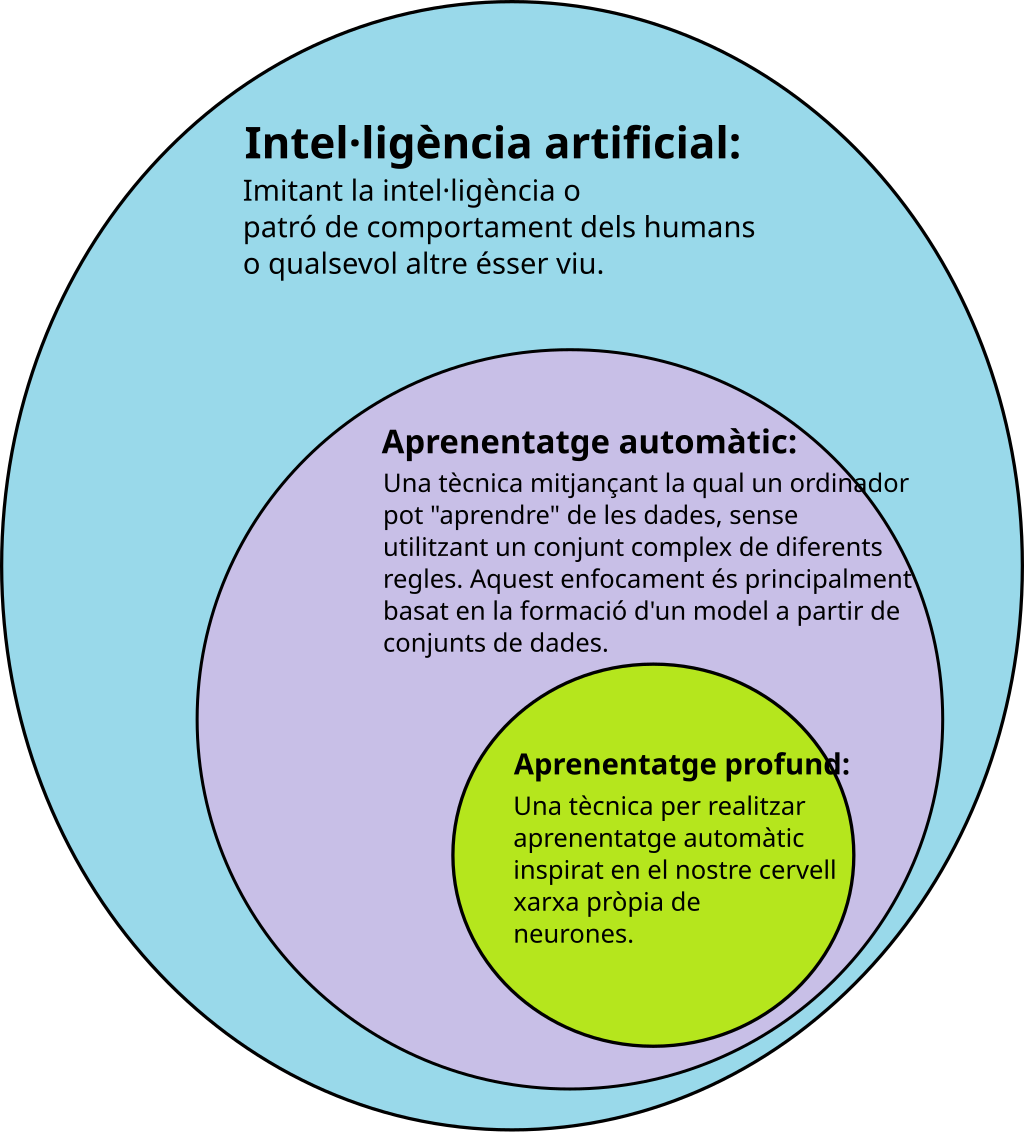
\includegraphics[width=0.2\textwidth]{./figures/Aprenentatge.png}
    \caption{Les capes que te la IA per funcionar}
    \end{figure}
          \end{enumerate}

  \item \textbf{Frameworks}
      Segons INESDI~\cite{INESDI}:\\
      {\color{gray}``Un Frameworks és, en el camp de la informàtica, una estructura conceptual que proporciona un conjunt d'eines, biblioteques i patrons de disseny per facilitar el desenvolupament de programari.
      %En altres paraules, són marcs de treball que funcionen com un esquelet predefinit, i sobre els quals es pot construir una aplicació o programari.

     Pel que fa als seus components, inclouen biblioteques de codi reutilitzables, mòduls predefinits, regles d'arxiu i directori, patrons de disseny i convencions de codificació.''}\\

      %Un Framework, en diferencia, de la biblioteca per el control total que pot tenir el usuari en tema estructura, i organitzacio dels codis, en canvi, una biblioteca està en mans del desenvolupador i només tens accés en els codis que et convenin de la biblioteca. Malgrat la utilitat que propociona no satisfeix la IA de la actualitat i han hagut de desarollar uns Frameworks especifics per la IA, de tal manera en que facilita el desarollament i l'entrenament dels models de la IA.

     \item \textbf{Ètica i Regulació}\\
      Un cop enteses totes les funcionalitats i capacitats de la intel·ligència artificial (IA), és fonamental aplicar-hi principis d’ètica i moral. Encara que la IA no sigui un ésser viu, és una eina creada per els  humans, i per tant cal establir-hi limitacions per evitar-ne els mals usos i garantir el respecte als drets humans i a la privacitat. Aquesta part és crucial en el desenvolupament d’una IA responsable. En aquest sentit, molts estats i organismes ja han publicat diverses lleis legítimes i regulacions. Algunes de les més rellevants són:
     \begin{itemize}
        \item \textbf{Llei d’IA de la Unió Europea (AI Act):} És la primera regulació integral sobre la IA. Classifica els sistemes d’IA segons el seu nivell de risc (inacceptable, alt, limitat i mínim) i estableix requisits estrictes per als usos d’alt risc, com la transparència, supervisió humana i seguretat.
           \item \textbf{Reglament General de Protecció de Dades (GDPR):} Tot i no ser exclusiu per a la IA, aquest reglament europeu protegeix la privacitat i les dades personals dels ciutadans. És clau en el desenvolupament d’IA que utilitza dades personals.
          \item \textbf{Principis ètics de la UNESCO sobre la IA (2021): Proposen una base global per al desenvolupament ètic de la IA, centrant-se en el respecte pels drets humans, la igualtat, la sostenibilitat, la no discriminació i la supervisió humana.}
          \item \textbf{Guies de l’OCDE sobre la IA:}Recomanen que els sistemes d’IA siguin transparents, responsables, segurs i que promoguin el benestar de la societat, ajudant a establir marcs internacionals de bones pràctiques.
     \end{itemize}


 \end{enumerate}





Fonts:~\cite{Universitat_oberta_catalunya},~\cite{Generalitat},~\cite{IBM_machine_learning},~\cite{Ultralytics},~\cite{bengio2012},~\cite{Ai_Act}, \cite{Algorismes} i ~\cite{Unesco}.

\section{Que és una xarxa neuronal artificial/biologica?}\label{sec:xarxa neuronal}
Una xarxa neuronal artificial és un model computacional inspirat en el funcionament del cervell humà, utilitzat en el camp de la intel·ligència artificial (IA) i l'aprenentatge automàtic (machine learning). Està dissenyada per reconèixer patrons, prendre decisions i aprendre a partir de dades, sense ser programada explícitament per a cada tasca específica.\\ \\
Si tenim una artificial també tindrem una biològica. Una xarxa neuronal biològica es refereix al sistema interconnectat de neurones (cèl·lules nervioses) en el cervell i el sistema nerviós dels éssers vius. Aquestes xarxes són la base de la cognició, l'aprenentatge i les funcions biològiques en humans i animals.\\


\section{Estructura d'una xarxa neuronal}\label{sec:3.6}
Una xarxa neuronal combina diverses capes de processament i utilitza elements simples que operen en paral·lel, simulen i estan inspirades en els sistemes nerviosos biològics com hem explicat en l'apartat \ref{sec:xarxa neuronal}. Consta d'una capa d'entrada, seguit d'una o diverses capes ocultes i finalment una capa de sortida. Les capes estan interconnectades mitjançant nodes o neurones; cada capa utilitza la sortida de la capa anterior com a entrada.

\begin{itemize}
 \item \textbf{Capa d'entrada:}La capa d'entrada és la primera capa que rep directament la informació d'entrada que es processarà.
 \item \textbf{Capes ocultes:}Les capes ocultes són les capes que estan entre la capa d'entrada i la de sortida, aquestes capes contenen unitats no observables. La seva funció principal és processar les dades de la capa d'entrada per extraure característiques i patrons complexos.  La quantitat de neurones que hi ha en les capes ocultes és un factor determinant per la capacitat que tingui la xarxa per capturar dades complexes.
 \item \textbf{Capa de sortida:}La capa de sortida és l'última capa que forma una xarxa neuronal i és l'encarregada de produir la predicció o el resultat final del model. Aquesta capa utilitza la informació que ha processat la o les capes ocultes i la transforma a través d'una funció activa per generar una sortida, que pot ser una predicció numèrica, una classificació o qualsevol altre resultat. Les neurones d'aquesta capa estan connectades amb totes les neurones de la capa anterior.
 \end{itemize}


\begin{figure}[h!]
    \centering
    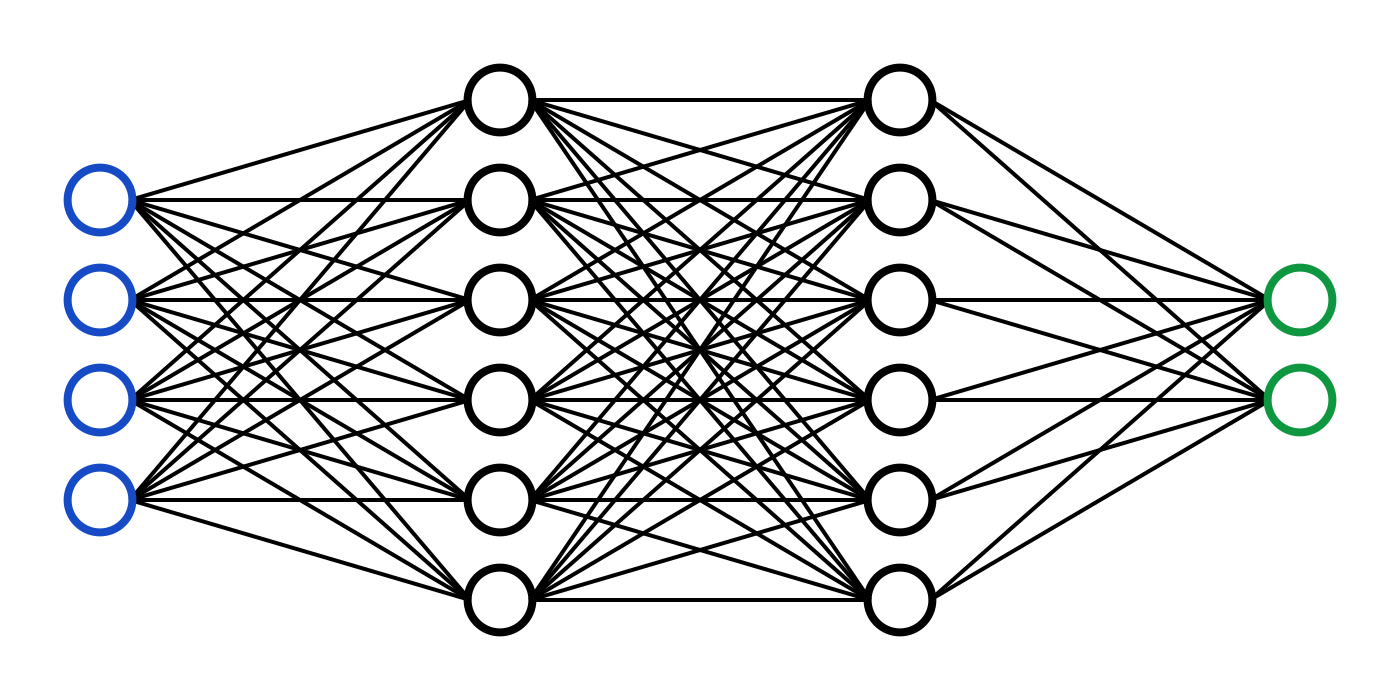
\includegraphics[width=0.5\textwidth]{./figures/xarxa.png}
    \caption{Estructura d'una xarxa neuronal}
\end{figure}

Fonts:~\cite{Hidden_layer} i~\cite{linkedin}

\section{Exemples de xarxes neuronals}
Hi ha molts tipus de xarxes neuronals, però com que el treball té una limitació de pàgines farem un resum de les xarxes més rellevants.

\begin{enumerate}
    \item \textbf{Perceptron (1958)}

    La primera xarxa neuronal, el Perceptró, va ser creada en la dècada de 1950 a 1960 pel psicòleg i informàtic Frank Rosenberg. Aquesta màquina permet prendre decisions binàries, per exemple respondre sí o no, de manera autònoma. \\
%     Aquest model pren varies entrades binaries $x_1$, $x_2$, fins les que calguin, i produeix una sola sortida binaria. Per calcular la sortida, Rosenblatt va introduir els ``pesos'', que está explicat a l'apartat \ref{sec:3.8}, els seus principals usos són decsions binàries senziles, o per crear funcions lògiques com OR o AND.
%%%%%%%%%%%%%% Això ho heu de simplificar molt, no cal entrar en tants detalls, feu com jo he fet a l'apartat anterior
    \item \textbf{Multiplayer Perceptron}
    El multiplayer perceptron és una ampliació de la percepció d'una única neurona a més d'una. A més, apareix el concepte de capes d'entrades, capes ocultes i capes de sortida, però amb valors d'entrada i sortida binàries.\\
    \item \textbf{Neurones sigmoide}
    Per aconseguir que les xarxes neuronals aprenguin per elles mateixes, és a dir, aprenentatge automàtic \ref{Aprenentatge_automàtic}, va ser necessari introduir un nou tipus de neurones, que són les Neurones Sigmoides, que són similars al perceptró, aquestes neurones en comptes de què les entrades siguin 1 o 0, puguin tenir valors com 0.5, o 0.374 o qualsevol altre valor real.\\

    %Ara les sorides en lloc de ser 0 o 1, serà d(w . x + b), on d serà la funció sigmoide, explicat en l'apartat \ref{sigmoide}. Aquesta va ser la primera funció d'activació \ref{Activació}.

    \item \textbf{Xarxa neuronal prealmentada (Feedforward)}
    Les xarxes neuronals prealimentades són les que les sortides d'una sola capa són utilitzades com entrades en la pròxima.
\end{enumerate}

\section{
Funció d'activació}\label{Activació}
Les funcions d'activació són un component integral de les xarxes neuronals que els permeten aprendre patrons complexos en les dades. Transformen el senyal d'entrada d'una neurona en un senyal de sortida que passa a la capa següent. Sense funcions d'activació, les xarxes neuronals es limitarien a modelar únicament relacions lineals entre entrades i sortides, és a dir, introdueixen la no-linealitat i produeixen la sortida de la neurona.

\begin{enumerate}
 \item \label{sigmoide}{\textbf{Funció sigmoide}}\\
 Una funció d'activació molt coneguda és la funció sigmoide. La seva fórmula és:
$$[ \sigma(x) = \frac{1}{1 + e^{-x}} ]$$

Aquesta funció matemàtica transforma qualsevol valor d'entrada real en un valor que està 0 i 1. La seva forma característica és una corba en forma de ``S''. Si el valor de $x$ que introduïm a la funció és molt gran o fins infinit $(\infty)$, llavors\ $\sigma$ serà 1; en canvi, si és molt petit o menys infinit $(-\infty)$,\ $\sigma$ serà 0, i si x = 0,  $\sigma$  serà 0,5.

\begin{figure}[h!]
    \centering
    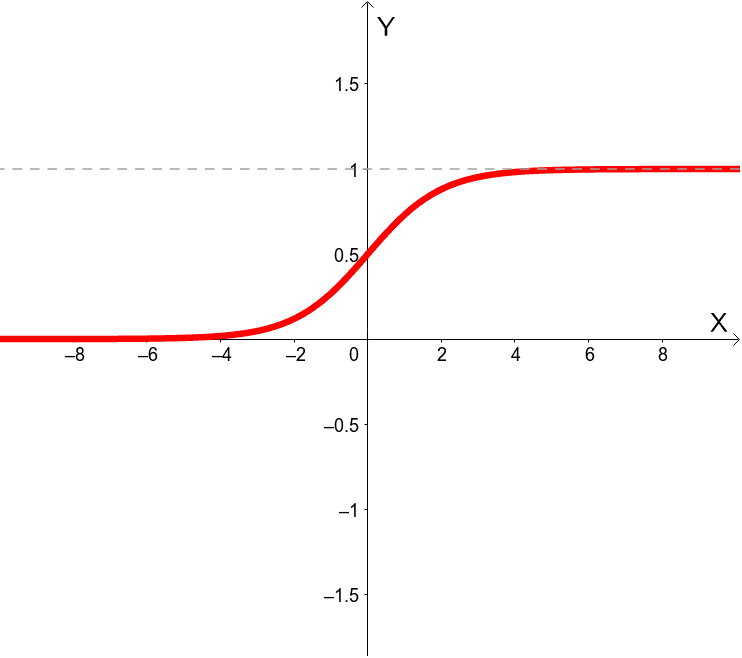
\includegraphics[width=0.5\textwidth]{./figures/grafica_sigmoide.png}
    \caption{Gràfica de la funció sigmoide}
\end{figure}
\begin{comment}
\textbf{Avantatges:}
La avantatge principal de la funció sigmoide és la seva suavitat i la facilitat de derivació. La funció és diferenciable en tots els punts, cosa que facilita el càlcul de gradients, això vol dir que permet als algoritmes d'optimització treballar amb la funció de manera eficient. A més, la funció és monòtona creixent, ho que significa que una entrada major sempre produirà una sortida major, fent que sigui útil per modelar relacions de causa i efecte.

\textbf{Desavantatges:}
Tanmateix, la funció sigmoide també té algunes desavantatges. Un dels seus problemes és que la funció es satura els gradients. Quan els valors d'entrades són grans, ho que significa que la derivada de la funció s'apropa a 0 i l'aprenentatge es relentitza. Un altre problema és que aquesta funció no és simètrica, causant a les entrades negatives i positives es processin de mandera diferent, això pot afectaral rendiment de la xarxa. Tot això dificulta el procès d'entrenament de la xarxa en la ràpida minimització de la funció d'error utilitzant l'algoritme de Gradient Descendent.
\end{comment}
\item \hypertarget{subsec:1}{\textbf{Funció ReLU(Funció Uniat Rectificada Uniforme)}}\\

La funció Unitat Rectificada Uniforme té la fòrmula seguent:
\[ f(x) = \max(0, x) \]

Aquesta funció té l'algoritme següent: Si el valor d'entrada és menor que 0, en mostra 0, si el valor d'entrada és major o igual que 0, mostrarà el valor d'entrada. Això vol dir que la funció és lineal si l'entrada és més gran que 0 perquè el pendent és 1. Encara que la funció ReLU és lineal per a la meitat del seu espai d'entrada, tècnicament és una funció no lineal perquè té un punt no diferenciable en x = 0, on canvia bruscament respecte a x. Aquesta no-linealitat permet a les xarxes neuronals aprendre patrons complexos.

\begin{figure}[h!]
    \centering
    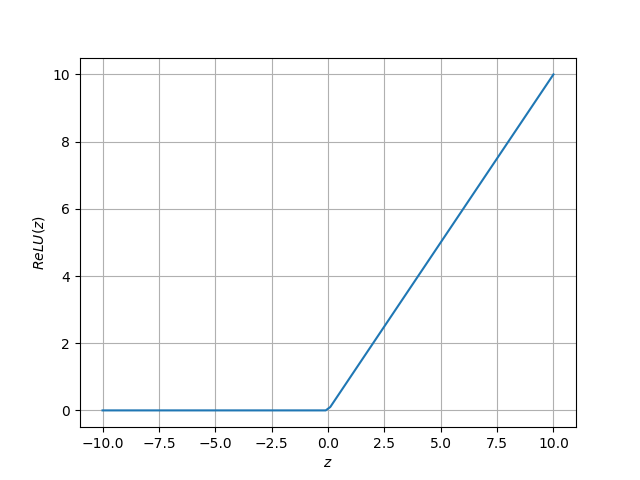
\includegraphics[width=0.5\textwidth]{./figures/ReLU.png}
    \caption{Gràfica de la funció ReLU}
\end{figure}
\begin{comment}
Tot i això, aquesta funció té una desavanantatge; si utilitzen la funció ReLU com a funció d'activació pasarà una cosa, i es que tots els valors negatius són 0, per tant en el procès de retropropagació, explicat a l'apartat \ref{subsec:retropropagació}, no es produeix els valors d'ajust en les neurones negatives. Per solucionar aquest problema s'ha inventat una nova funció que es diu Leaky ReLU. Funciona igual com l funció ReLU, però té un valor determinat per les neurones negatives.

\begin{figure}[h!]
    \centering
    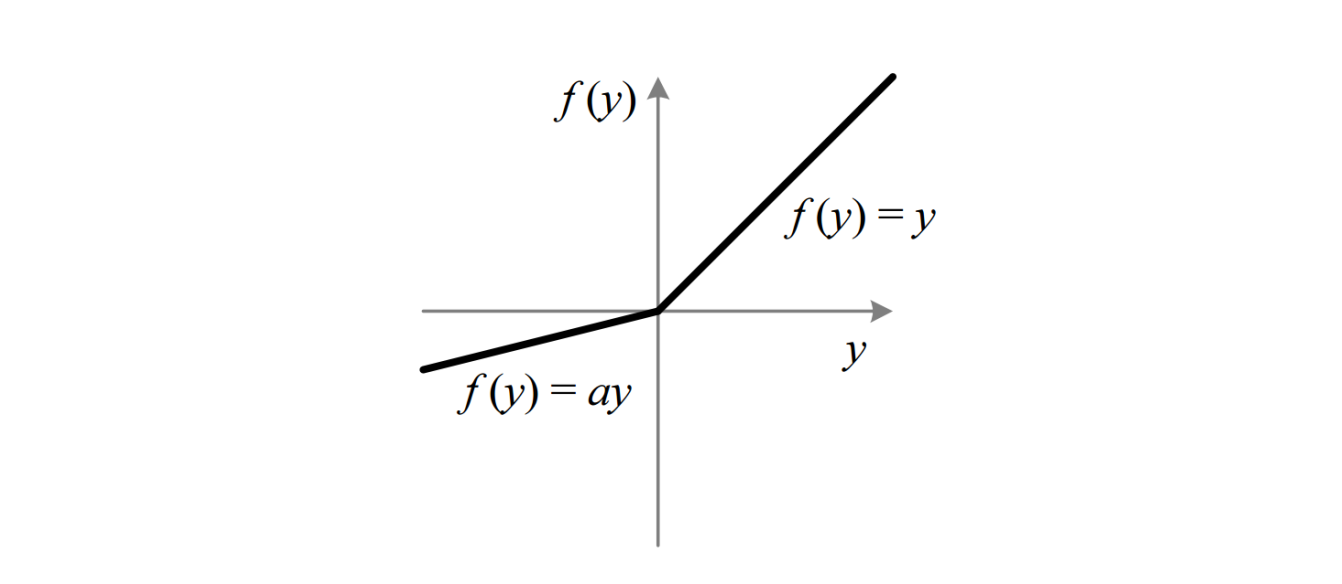
\includegraphics[width=0.5\textwidth]{./figures/leaky_ReLU.png}
    \caption{Gràfica de la funció Leaky ReLU}
\end{figure}
\end{comment}

\item \textbf{Funció Softmax}\\

La funció Softmax és una de les funcions que més s'utilitzen en xarxes neuronals i és especialment útil en el context dels problemes de classificació multiclasse. Aquesta funció opera sobre un vector que representa les previsions de cada classe, calculades per les capes anteriors.

\begin{figure}[h!]
    \centering
    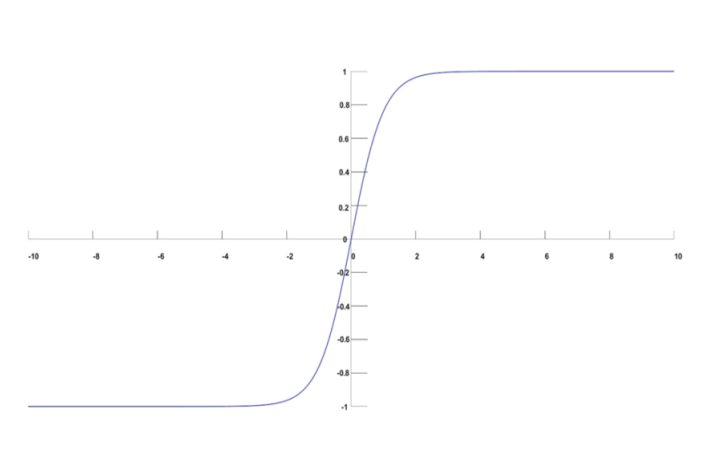
\includegraphics[width=0.5\textwidth]{./figures/Softmax.png}
    \caption{Gràfica de la funció Softmax}
\end{figure}

Per a un vector d'entrada x amb elements x1, x2,..., xC, la funció Softmax es defineix com:
$$[f(x_i) = \frac{e^{x_i}}{\sum_{j=1}^{n} e^{x_j}}]$$

El resultat de la funció Softmax és una distribució de probabilitat de la qual la suma és 1. Cada element del resultat representa la probabilitat que l'entrada pertanyi a una classe determinada. L'ús d'aquesta funció garanteix que tots els valors de la sortida siguin positius. Això és molt important perquè les probabilitats no poden ser negatives.

\begin{figure}[H]
    \centering
    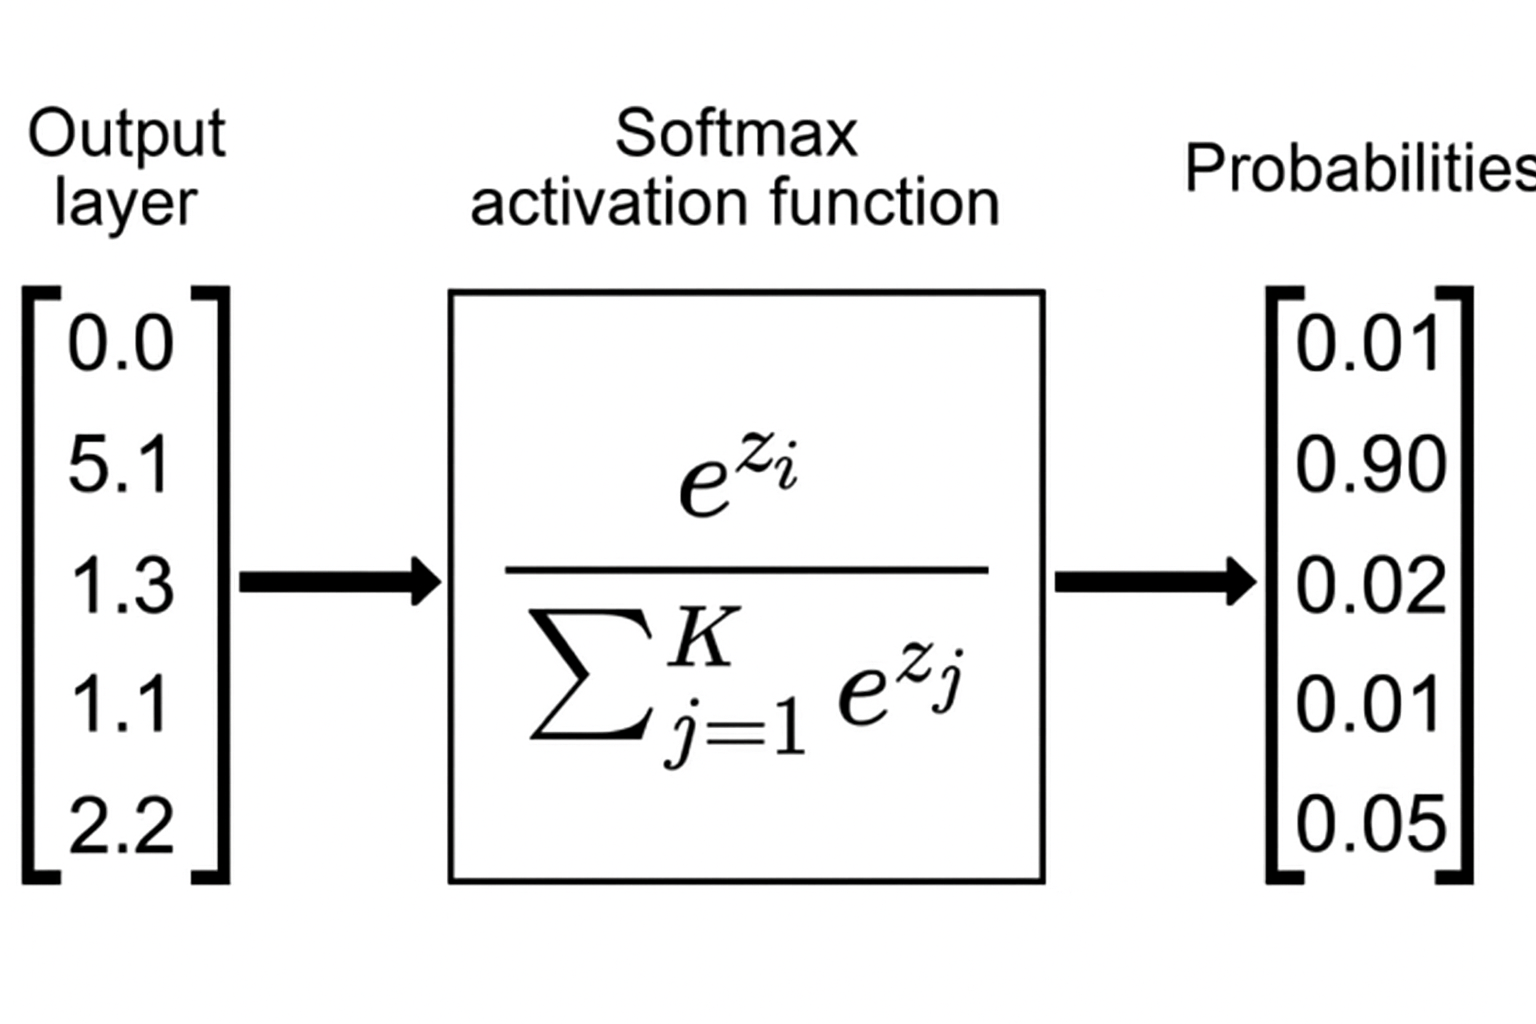
\includegraphics[width=0.5\textwidth]{./figures/representacio_Softmax.png}
    \caption{Representació de la funció Softmax}
\end{figure}

Fonts: ~\cite{Hidden_layer} i~\cite{Jacar}
\end{enumerate}

\section{Com funciona una xarxa neuronal?}\label{sec:3.8}
Ara que sabem quina estructura forma una xarxa neuronal artificial, toca entendre com funciona. Les neurones o nodes són els pilars més importants d'una xarxa neuronal. Cada neurona utilitza l'entrada, la processa fent una suma ponderada entre els pesos i les entrades, després una funció d'activació, i passa la sortida a altres neurones.\\

Les conexions (pesos i biaixos) són la força de connexió entre dues neurones representades per un pes.
\textbf{Els pesos:} Són valors que determinen quanta influència té la producció d'una neurona sobre un altre, marca la importància que té cada neurona.\\

Els biaixos: Són paràmetres addicionals que ajuda a ajustar els valors de les neurones. És un valor capaç d'aprendre com el pes, això vol dir que el model pot utilitzar l'algoritme de retropropagació per a millorar els valors com per exemple els pesos i biaixos.

El umbral: Si la sortida de qualsevol node individual és més gran que el valor del umbral, aquell node s'activarà i envia dades a la següent capa de la xarxa. En cas contrari, no passarà cap dada a la següent capa de la xarxa.\\

Hem de pensar en què cada node individual com el seu propi model de regressió lineal, compost per dades d'entrada, ponderacions, un umbral o un biaix, i una sortida. La fórmula per calcular els valors d'una xarxa neuronal és la següent:

$$[
\sum w_i x_i + \text{biaix} = w_1 x_1 + w_2 x_2 + w_3 x_3 + \text{biaix}
]$$ \\

$w_i$: Pesos\\
$x_i$: Entrades\\

\begin{comment}
Per entendre-ho millor, donarem un exemple: Imagina que vols anar a la platja a fer surf i la teva decisió dependrà d'aquestes 3 preguntes:\\

Hi ha oles?\\
Hi ha poca gent?\\
Hi ha tauros?\\

Analitzarem en detall com funciona un sol node de la xarxa neronal, utilitzant únicament valors binaris (0 y 1) com entrades, 0 voldrà dir ``No'' y 1 ``sí''.
LLavors suposent el següent cas:

$x_1$ = 1, les oles són bones\\
$x_2$ = 0, hi ha molta gent a la platja\\
$x_3$ = 1, Sí que tinc temps\\

Ara, hem d'asignar algunes ponderacions per determinar la importància. Unes ponderacions majors significan que determinades variabbles son més importants per la decisió.

$w_1$ = 5, hi ha d'haveri moltes oles per poder surfejar\\
$w_2$ = 2, no t'importa que hi hagi molta gent\\
$w_3$ = 4, tens pors als taurons \\

Per últim, ambé suposem un valor umbral de 3, ho que es traduiria en un valor de biaix de -3. Amb totes aquestes entrades, ja podem substituir els valors en la nostre fòrmula per obtenir la sortida.
\end{comment}

Fonts: \cite{IMB_Xarxa_neuronal}
%\href{https://aws.amazon.com/es/what-is/neural-network/}{Amazon Web Services} Aquesta pàgina ja no existeix

\subsection{Propagació cap a davant}\label{subsec:propagació}
Durant la propagació cap a davant, les dades ingressen en la xarxa a través de la capa d'entrada i flueixen seqüencialment a través de les capes ocultes fins a la capa de sortida. En cada neurona, els valors d'entrada del model es multipliquen pels seus pesos corresponents i se sumen. Aquesta suma ponderada passarà a través d'una funció d'activació, explicada prèviament a l'apartat \ref{Activació}. Aquest procés continua capa per capa, això acaba conduint cap a la predicció final en la capa de sortida.

Aquest procés és important per les següents raons:
\begin{itemize}
 \item \textbf{Base per l'aprenentatge:} No es pot comprendre com aprenen les xarxes neuronals sense primer entendre com fan prediccions. La programació cap a davant és el requisit previ que s'ha de conèixer per comprendre la \nameref{subsec:retropropagació}, l'algoritme que permet l'aprenentatge.

 \item \textbf{Optimització:} En el cas que una xarxa neuronal no funcioni bé, saber com flueixen les dades per la xarxa t'ajudarà a identificar i solucionar problemes.

 \item \textbf{Disseny del model:} Un disseny eficaç de la xarxa requereix comprendre com es distribueix la informació a través de les configuracions de capes.
\end{itemize}

\section{Retropropagació en les xarxes neuronals}\label{subsec:retropropagació}
Mentre que la programació directa fa prediccions, la retropropagació és la forma en què la xarxa aprèn d'errors. Implica comparar la predicció de la xarxa amb el valor objectiu real i calcular un terme d'error mitjançant una funció d'error.\\
Aquest error es propaga enrere a través de la xarxa, començant des de la capa de sortida. Durant aquest procés, la xarxa ajusta els pesos i els biaixos de cada connexió en funció de la seva contribució a l'error, amb l'objectiu de minimitzar-lo.\\
Aquest procés iteratiu de càlcul d'erros i ajustament de pes permet a la xarxa d'aprenentatge profund millorar gradualment les seves prediccions.\\
El procés de retropropagació es basa en el principi d'optimització del gradient descendent, explicat anteriorment en l'apartat \ref{Algoritme_gradient}, es calculen els gradients d'error respecte als paràmetres de la xarxa en sentit contrari i en cada capa. Per aquesta tasca, s'utilitza l'algoritme de la cadena per propagar l'error cap endarrere des de la sortida fins a l'entrada.

\subsection{Com funcona la retropropagació?}
El funcionament de la retropropagació el podem dividir en 5 fases. Cada una d'aquestes possibilita a la xarxa neuronal aprendre de manera eficient a partir de dades proporcionades. Les fases són les següents:

\begin{itemize}

 \item \textbf{Propagació cap endavant:} Aquesta fase inicial és on s'introdueixen les dades de prova en la xarxa neuronal des de la capa d'entrada fins a la sortida.

 \item \textbf{Càlcul d'error:} Una vegada s'obté la sortida de la xarxa, es compara amb el valor desitjat mitjançant una funció d'error. Aquesta funció quantifica la discrepància que s'ha produït entre la predicció i el valor real.

 \item \textbf{Retropropagació de l'error:} En aquesta fase els gradients de l'error es calculen respecte a cada paràmetre en la xarxa. Com hem dit abans, aquest procés comença de manera inversa a la propagació, des de la sortida fins a l'entrada.

 \item \textbf{Actualització dels paràmetres:} Una vegada que s'ha calculat els gradients de l'error en tots els paràmetres, aquests s'actualitzen. D'aquesta manera, els errors en la predicció es minimitzen de manera gradual en cada iteració de l'entrenament.

 \item \textbf{Configuració de la predicció:} Després de totes les optimitzacions, el mètode de càlcul torna a revisar les entrades de prova. Després de tot això, es busca garantir els resultats esperats.
\end{itemize}
\begin{comment}
\subsection{Avantatges de la retropropagació}
La retropropagació ofereix unes avantatges que l'han convertit en una eina fonamental en l'entrenament de les xarxes neuronals. Les seves avantatges són les seguents:

\begin{itemize}
 \item \textbf{Eficiència en l'optimització de parámetres:} Gracies al càlcul de gradient mitjantçant la regla de la cadena, explicada a l'apartat \ref{subsec:cadena}, la retropropagació facilita l'ajust dels paràmetres d'una xarxa neuronal de manera eficient. Això s'aconsegueix determinant la contribució de cada variable al error total de la xarxa, ho que augmenta notablement a l'hora de fer prediccions precises.
 \item \textbf{Flexibilitat en l'arquitectura:} La retropropagació és compatible en moltes varietats d'arquitectura en les xarxes neuronals, com l'aprenentatge profund amb múltiples capes ocultes. Aquesta característica permet disenys que s'adapten millor a la complexitat de dades i les necesitats de cada tasca.
 \item \textbf{Escalabilitat:} Es posible augmentar la retropropagació perquè traballi amb moltes dades i xarxes neuronas molt grans, ja que hi haurà vegades en que una xarxa pot tindre fins a milions de paràmetres, això exigeix una gestió eficient.
 \item \textbf{Optimització continua:} La retropropagació ofereix la actualització contínua de les variables durant l'entrenament. És un ajust dinàmic important per millorar poc a poc el rendiment de la xarxa amb cada iteració i nous cicles d'aprenentatges.
\end{itemize}
\end{comment}
Fonts: ~\cite{valencia} i~\cite{Retropropagacio}



